\documentclass[10pt]{article}
\usepackage[polish]{babel}
\usepackage[utf8]{inputenc}
\usepackage[T1]{fontenc}
\usepackage{amsmath}
\usepackage{amsfonts}
\usepackage{amssymb}
\usepackage[version=4]{mhchem}
\usepackage{stmaryrd}
\usepackage{graphicx}
\usepackage[export]{adjustbox}
\graphicspath{ {./images/} }

%New command to display footnote whose markers will always be hidden
\let\svthefootnote\thefootnote
\newcommand\blfootnotetext[1]{%
  \let\thefootnote\relax\footnote{#1}%
  \addtocounter{footnote}{-1}%
  \let\thefootnote\svthefootnote%
}

%Overriding the \footnotetext command to hide the marker if its value is `0`
\let\svfootnotetext\footnotetext
\renewcommand\footnotetext[2][?]{%
  \if\relax#1\relax%
    \ifnum\value{footnote}=0\blfootnotetext{#2}\else\svfootnotetext{#2}\fi%
  \else%
    \if?#1\ifnum\value{footnote}=0\blfootnotetext{#2}\else\svfootnotetext{#2}\fi%
    \else\svfootnotetext[#1]{#2}\fi%
  \fi
}

\newcommand\Varangle{\mathop{{<\!\!\!\!\!\text{\small)}}\:}\nolimits}

\begin{document}
\section*{CENTRALNA \\
 KOMISJA \\
 EGZAMINACYJNA}
\begin{center}
\begin{tabular}{|c|c|}
\hline
Rodzaj dokumentu: & Zasady oceniania rozwiązań zadań \\
\hline
Egzamin: & Egzamin maturalny \\
\hline
Przedmiot: & Matematyka \\
\hline
Poziom: & Poziom podstawowy \\
\hline
Formy arkusza: & \begin{tabular}{l}
EMAP-P0-100 (wersje arkusza: A i B), EMAP-P0-200, EMAP-P0-300, \\
EMAP-P0-400, EMAP-P0-600, \\
EMAP-P0-700, EMAP-P0-K00, \\
EMAP-P0-Q00, EMAU-P0-100 \\
\end{tabular} \\
\hline
Termin egzaminu: & 8 maja 2024 r. \\
\hline
Data publikacji dokumentu: & 28 czerwca 2024 r. \\
\hline
\end{tabular}
\end{center}

\section*{Uwaga:}
Gdy wymaganie egzaminacyjne dotyczy treści z III etapu edukacyjnego, dopisano „G".

\section*{ZADANIA ZAMKNIETE}
Zadanie 1. (0-1)

\begin{center}
\begin{tabular}{|l|l|}
\hline
\multicolumn{2}{|c|}{Wymagania egzaminacyjne 20241} \\
\hline
\multicolumn{1}{|c|}{Wymaganie ogólne} & \multicolumn{1}{|c|}{Wymaganie szczegółowe $^{|c|}$\begin{tabular}{l}
Zdajacy: \\
I. Wykorzystanie i tworzenie informacji. \\
\end{tabular}}\begin{tabular}{l}
1.8) wykonuje obliczenia procentowe [...]. \\
\end{tabular} \\
\hline
\end{tabular}
\end{center}

\section*{Zasady oceniania}
1 pkt - odpowiedź poprawna.\\
0 pkt - odpowiedź niepoprawna albo brak odpowiedzi.

\section*{Rozwiązanie}
Wersja A

\section*{Wersja B}
C\\
B

\section*{Zadanie 2. (0-1)}
\begin{center}
\begin{tabular}{|l|l|}
\hline
\multicolumn{2}{|c|}{Wymagania egzaminacyjne 2024} \\
\hline
\multicolumn{1}{|c|}{Wymaganie ogólne} & \multicolumn{1}{c|}{Wymaganie szczegółowe} \\
\hline
II. Wykorzystanie i interpretowanie & Zdający: \\
reprezentacji. & \begin{tabular}{l}
1.4) oblicza potęgi o wykładnikach \\
 \\
 \\
 \\
 \\
 \\
 \\
wymiernych i stosuje prawa działań na \\
potęgach o wykładnikach wymiernych. \\
\hline
\end{tabular} \\
\hline
\end{tabular}
\end{center}

\section*{Zasady oceniania}
1 pkt - odpowiedź poprawna.\\
0 pkt - odpowiedź niepoprawna albo brak odpowiedzi.

\section*{Rozwiązanie}
Wersja A\\
Wersja B\\
B\\
C

\footnotetext{${ }^{1}$ Rozporządzenie Ministra Edukacji i Nauki z dnia 1 sierpnia 2022 r. w sprawie wymagań egzaminacyjnych dla egzaminu maturalnego przeprowadzanego w roku szkolnym 2022/2023 i 2023/2024 (Dz.U. 2022, poz.1698).
}\section*{Zadanie 3. (0-1)}
\begin{center}
\begin{tabular}{|l|l|}
\hline
\multicolumn{2}{|c|}{Wymagania egzaminacyjne 2024} \\
\hline
\multicolumn{1}{|c|}{Wymaganie ogólne} & \multicolumn{1}{c|}{Wymaganie szczegółowe} \\
\hline
\begin{tabular}{l}
II. Wykorzystanie i interpretowanie \\
reprezentacji. \\
\end{tabular} & \begin{tabular}{l}
Zdajacy: \\
1.6) wykorzystuje definicję logarytmu [...]. \\
\end{tabular} \\
\hline
\end{tabular}
\end{center}

\section*{Zasady oceniania}
1 pkt - odpowiedź poprawna.\\
0 pkt - odpowiedź niepoprawna albo brak odpowiedzi.

\section*{Rozwiązanie}
Wersja A\\
C

Wersja B\\
B

\section*{Zadanie 4. (0-1)}
\begin{center}
\begin{tabular}{|l|l|}
\hline
\multicolumn{2}{|c|}{Wymagania egzaminacyjne 2024} \\
\hline
\multicolumn{1}{|c|}{Wymaganie ogólne} & \multicolumn{1}{c|}{Wymaganie szczegółowe} \\
\hline
II. Wykorzystanie i interpretowanie & Zdajacy: \\
reprezentacji. & 2. używa wzorów skróconego mnożenia na \\
 & $(a \pm b)^{2}$ oraz $a^{2}-b^{2}$. \\
\hline
\end{tabular}
\end{center}

\section*{Zasady oceniania}
1 pkt - odpowiedź poprawna.\\
0 pkt - odpowiedź niepoprawna albo brak odpowiedzi.

\section*{Rozwiązanie}
Wersja A\\
Wersja B\\
B\\
D

\section*{Zadanie 5. (0-1)}
\begin{center}
\begin{tabular}{|l|l|}
\hline
\multicolumn{2}{|c|}{Wymagania egzaminacyjne 2024} \\
\hline
\multicolumn{1}{|c|}{Wymaganie ogólne} & \multicolumn{1}{c|}{Wymaganie szczegółowe} \\
\hline
\begin{tabular}{l}
II. Wykorzystanie i interpretowanie \\
reprezentacji. \\
\end{tabular} & \begin{tabular}{l}
Zdający: \\
 \\
\hline
\end{tabular} \\
\hline
\end{tabular}
\end{center}

\section*{Zasady oceniania}
1 pkt - odpowiedź poprawna.\\
0 pkt - odpowiedź niepoprawna albo brak odpowiedzi.

\section*{Rozwiązanie}
Wersja A Wersja B\\
D D

Zadanie 6. (0-1)

\begin{center}
\begin{tabular}{|l|l|}
\hline
\multicolumn{2}{|c|}{Wymagania egzaminacyjne 2024} \\
\hline
\multicolumn{1}{|c|}{Wymaganie ogólne} & \multicolumn{1}{c|}{Wymaganie szczegółowe} \\
\hline
II. Wykorzystanie i interpretowanie & Zdający: \\
reprezentacji. & 3.6) korzysta z własności iloczynu przy \\
 & rozwiązywaniu równań typu \\
 & $x(x+1)(x-7)=0$. \\
\hline
\end{tabular}
\end{center}

\section*{Zasady oceniania}
1 pkt - odpowiedź poprawna.\\
0 pkt - odpowiedź niepoprawna albo brak odpowiedzi.

\section*{Rozwiązanie}
Wersja A\\
B

Wersja B\\
C

\section*{Zadanie 7. (0-1)}
\begin{center}
\begin{tabular}{|l|l|}
\hline
\multicolumn{2}{|c|}{Wymagania egzaminacyjne 2024} \\
\hline
\multicolumn{1}{|c|}{Wymaganie ogólne} & \multicolumn{1}{c|}{Wymaganie szczegółowe} \\
\hline
II. Wykorzystanie i interpretowanie & \begin{tabular}{l}
Zdający: \\
reprezentacji. \\
\end{tabular} \\
 & \begin{tabular}{l}
3.7) rozwiązuje proste równania wymierne, \\
prowadzące do równań liniowych lub \\
kwadratowych [...]. \\
\end{tabular} \\
\hline
\end{tabular}
\end{center}

\section*{Zasady oceniania}
1 pkt - odpowiedź poprawna.\\
0 pkt - odpowiedź niepoprawna albo brak odpowiedzi.

\section*{Rozwiązanie}
Wersja A\\
Wersja B\\
B\\
B

\section*{Zadanie 8. (0-1)}
\begin{center}
\begin{tabular}{|l|l|}
\hline
\multicolumn{2}{|c|}{Wymagania egzaminacyjne 2024} \\
\hline
\multicolumn{1}{|c|}{Wymaganie ogólne} & \multicolumn{1}{c|}{Wymaganie szczegółowe} \\
\hline
II. Wykorzystanie i interpretowanie & Zdający: \\
reprezentacji. & G7.7) za pomocą równań lub układów \\
 & równań opisuje i rozwiązuje zadania \\
 & osadzone w kontekście praktycznym. \\
\hline
\end{tabular}
\end{center}

\section*{Zasady oceniania}
1 pkt - odpowiedź poprawna.\\
0 pkt - odpowiedź niepoprawna albo brak odpowiedzi.

\section*{Rozwiązanie}
Wersja A\\
A

Wersja B\\
D

\section*{Zadanie 9. (0-1)}
\begin{center}
\begin{tabular}{|l|l|}
\hline
\multicolumn{2}{|c|}{Wymagania egzaminacyjne 2024} \\
\hline
Wymaganie ogólne & \multicolumn{1}{c|}{Wymaganie szczegółowe} \\
\hline
V. Rozumowanie i argumentacja. & \begin{tabular}{l}
Zdający: \\
G9.3) wyznacza średnią arytmetyczną [...] \\
zestawu danych. \\
\end{tabular} \\
\hline
\end{tabular}
\end{center}

\section*{Zasady oceniania}
1 pkt - odpowiedź poprawna.\\
0 pkt - odpowiedź niepoprawna albo brak odpowiedzi.

\section*{Rozwiązanie}
Wersja A Wersja B\\
A\\
C

Zadanie 10. (0-1)

\begin{center}
\begin{tabular}{|l|l|}
\hline
\multicolumn{2}{|c|}{Wymagania egzaminacyjne 2024} \\
\hline
\multicolumn{1}{|c|}{Wymaganie ogólne} & \multicolumn{1}{c|}{Wymaganie szczegółowe} \\
\hline
I. Wykorzystanie i tworzenie informacji. & \begin{tabular}{l}
Zdający: \\
3.2) wykorzystuje interpretację \\
geometryczną układu równań stopnia \\
pierwszego z dwiema niewiadomymi. \\
\end{tabular} \\
\hline
\end{tabular}
\end{center}

\section*{Zasady oceniania}
1 pkt - odpowiedź poprawna.\\
0 pkt - odpowiedź niepoprawna albo brak odpowiedzi.

\section*{Rozwiązanie}
Wersja A\\
Wersja B\\
A\\
C

Zadanie 11. (0-1)

\begin{center}
\begin{tabular}{|l|l|}
\hline
\multicolumn{2}{|c|}{Wymagania egzaminacyjne 2024} \\
\hline
\multicolumn{1}{|c|}{Wymaganie ogólne} & \multicolumn{1}{c|}{Wymaganie szczegółowe} \\
\hline
I. Wykorzystanie i tworzenie informacji. & \begin{tabular}{l}
Zdający: \\
 \\
 \\
 \\
\hline
\end{tabular} 4.3) odczytuje z wykresu własności funkcji \\
([...] zbiór wartości [...]). &  \\
\end{tabular}
\end{center}

\section*{Zasady oceniania}
1 pkt - odpowiedź poprawna.\\
0 pkt - odpowiedź niepoprawna albo brak odpowiedzi.

\section*{Rozwiązanie}
Wersja A\\
C

Wersja B\\
A

\section*{Zadanie 12. (0-1)}
\begin{center}
\begin{tabular}{|l|l|}
\hline
\multicolumn{2}{|c|}{Wymagania egzaminacyjne 2024} \\
\hline
\multicolumn{1}{|c|}{Wymaganie ogólne} & \multicolumn{1}{c|}{Wymaganie szczegółowe} \\
\hline
\multicolumn{1}{|c|}{II. Wykorzystanie i interpretowanie} & Zdający: \\
reprezentacji. & 4.7) interpretuje współczynniki występujące \\
 & we wzorze funkcji liniowej. \\
\hline
\end{tabular}
\end{center}

\section*{Zasady oceniania}
1 pkt - odpowiedź poprawna.\\
0 pkt - odpowiedź niepoprawna albo brak odpowiedzi.

\section*{Rozwiązanie}
Wersja A\\
Wersja B\\
B

Zadanie 13. (0-1)

\begin{center}
\begin{tabular}{|l|l|}
\hline
\multicolumn{2}{|c|}{Wymagania egzaminacyjne 2024} \\
\hline
\multicolumn{1}{|c|}{Wymaganie ogólne} & \multicolumn{1}{c|}{Wymaganie szczegółowe} \\
\hline
\begin{tabular}{ll}
II. Wykorzystanie i interpretowanie & \begin{tabular}{l}
Zdajacy: \\
reprezentacji. \\
\end{tabular} \\
\begin{tabular}{l}
4.6) wyznacza wzór funkcji liniowej na \\
podstawie informacji o funkcji lub o jej \\
wykresie. \\
\end{tabular} &  \\
\hline
\end{tabular} &  \\
\hline
\end{tabular}
\end{center}

\section*{Zasady oceniania}
1 pkt - odpowiedź poprawna.\\
0 pkt - odpowiedź niepoprawna albo brak odpowiedzi.

\section*{Rozwiązanie}
Wersja A\\
D

\section*{Wersja B}
A

\section*{Zadanie 14. (0-1)}
\begin{center}
\begin{tabular}{|l|l|}
\hline
\multicolumn{2}{|c|}{Wymagania egzaminacyjne 2024} \\
\hline
\multicolumn{1}{|c|}{Wymaganie ogólne} & \multicolumn{1}{c|}{Wymaganie szczegółowe} \\
\hline
I. Wykorzystanie i tworzenie informacji. & \begin{tabular}{l}
Zdający: \\
4.9) wyznacza wzór funkcji kwadratowej na \\
podstawie pewnych informacji o tej funkcji \\
lub o jej wykresie. \\
\end{tabular} \\
\hline
\end{tabular}
\end{center}

\section*{Zasady oceniania}
1 pkt - odpowiedź poprawna.\\
0 pkt - odpowiedź niepoprawna albo brak odpowiedzi.

\section*{Rozwiązanie}
Wersja A\\
B

Wersja B\\
A

Zadanie 15. (0-1)

\begin{center}
\begin{tabular}{|l|l|}
\hline
\multicolumn{2}{|c|}{Wymagania egzaminacyjne 2024} \\
\hline
\multicolumn{1}{|c|}{Wymaganie ogólne} & \multicolumn{1}{c|}{Wymaganie szczegółowe} \\
\hline
I. Wykorzystanie i tworzenie informacji. & \begin{tabular}{l}
Zdajacy: \\
 \\
 \\
\hline
\end{tabular}\begin{tabular}{l}
4.11) wykorzystuje własności funkcji [...] \\
kwadratowej [...]. \\
\end{tabular} \\
\hline
\end{tabular}
\end{center}

\section*{Zasady oceniania}
1 pkt - odpowiedź poprawna.\\
0 pkt - odpowiedź niepoprawna albo brak odpowiedzi.

\section*{Rozwiązanie}
Wersja A Wersja B\\
A\\
C

Zadanie 16. (0-1)

\begin{center}
\begin{tabular}{|l|l|}
\hline
\multicolumn{2}{|c|}{Wymagania egzaminacyjne 2024} \\
\hline
\multicolumn{1}{|c|}{Wymaganie ogólne} & \multicolumn{1}{|c|}{Wymaganie szczegółowe} \\
\hline
III. Modelowanie matematyczne. & \begin{tabular}{l}
Zdający: \\
 \\
 \\
 \\
 \\
 \\
5.3) stosuje wzór na $n$-ty wyraz [...] ciągu \\
arytmetycznego. \\
\end{tabular} \\
\hline
\end{tabular}
\end{center}

\section*{Zasady oceniania}
1 pkt - odpowiedź poprawna.\\
0 pkt - odpowiedź niepoprawna albo brak odpowiedzi.

\section*{Rozwiązanie}
Wersja A\\
C

Wersja B\\
C

\section*{Zadanie 17. (0-1)}
\begin{center}
\begin{tabular}{|l|l|}
\hline
\multicolumn{2}{|c|}{Wymagania egzaminacyjne 2024} \\
\hline
\multicolumn{1}{|c|}{Wymaganie ogólne} & \multicolumn{1}{|c|}{Wymaganie szczegółowe} \\
\hline
III. Modelowanie matematyczne. & Zdający: \\
 & \begin{tabular}{l}
5.4) stosuje wzór na $n$-ty wyraz [...] ciągu \\
geometrycznego. \\
\end{tabular} \\
\hline
\end{tabular}
\end{center}

\section*{Zasady oceniania}
1 pkt - odpowiedź poprawna.\\
0 pkt - odpowiedź niepoprawna albo brak odpowiedzi.

\section*{Rozwiązanie}
Wersja A\\
C

Wersja B\\
D

\section*{Zadanie 18. (0-1)}
\begin{center}
\begin{tabular}{|l|l|}
\hline
\multicolumn{2}{|c|}{Wymagania egzaminacyjne 2024} \\
\hline
\multicolumn{1}{|c|}{Wymaganie ogólne} & \multicolumn{1}{c|}{Wymaganie szczegółowe} \\
\hline
\begin{tabular}{ll}
\multicolumn{1}{|c|}{II. Wykorzystanie i interpretowanie} & Zdający: \\
reprezentacji. & 5.1) wyznacza wyrazy ciągu określonego \\
 & wzorem ogólnym. \\
\hline
\end{tabular} &  \\
\hline
\end{tabular}
\end{center}

\section*{Zasady oceniania}
1 pkt - odpowiedź poprawna.\\
0 pkt - odpowiedź niepoprawna albo brak odpowiedzi.

\section*{Rozwiązanie}
Wersja A\\
Wersja B\\
A\\
D

Zadanie 19. (0-1)

\begin{center}
\begin{tabular}{|l|l|}
\hline
\multicolumn{2}{|c|}{Wymagania egzaminacyjne 2024} \\
\hline
\multicolumn{1}{|c|}{Wymaganie ogólne} & \multicolumn{1}{|c|}{Wymaganie szczegółowe} \\
\hline
IV. Użycie i tworzenie strategii. & Zdający: \\
 & 6.3) stosuje proste zależności między \\
 & funkcjami trygonometrycznymi: \\
 & $\sin ^{2} \alpha+\cos ^{2} \alpha=1 \quad[\ldots]$. \\
\hline
\end{tabular}
\end{center}

\section*{Zasady oceniania}
1 pkt - odpowiedź poprawna.\\
0 pkt - odpowiedź niepoprawna albo brak odpowiedzi.

\section*{Rozwiązanie}
Wersja A\\
Wersja B\\
B\\
A

\section*{Zadanie 20. (0-1)}
\begin{center}
\begin{tabular}{|l|l|}
\hline
\multicolumn{2}{|c|}{Wymagania egzaminacyjne 2024} \\
\hline
\multicolumn{1}{|c|}{Wymaganie ogólne} & \multicolumn{1}{c|}{Wymaganie szczegółowe} \\
\hline
IV. Użycie i tworzenie strategii. & \begin{tabular}{l}
Zdający: \\
 \\
 \\
 \\
 \\
 \\
 \\
 \\
 \\
6.4) znając wartość jednej z funkcji: sinus \\
lub cosinus, wyznacza wartości pozostałych \\
funkcji tego samego kąta ostrego. \\
\end{tabular} \\
\hline
\end{tabular}
\end{center}

\section*{Zasady oceniania}
1 pkt - odpowiedź poprawna.\\
0 pkt - odpowiedź niepoprawna albo brak odpowiedzi.

\section*{Rozwiązanie}
Wersja A\\
B

\section*{Wersja B}
B

\section*{Zadanie 21. (0-1)}
\begin{center}
\begin{tabular}{|l|l|}
\hline
\multicolumn{2}{|c|}{Wymagania egzaminacyjne 2024} \\
\hline
\multicolumn{1}{|c|}{Wymaganie ogólne} & \multicolumn{1}{c|}{Wymaganie szczegółowe} \\
\hline
I. Wykorzystanie i tworzenie informacji. & Zdający: \\
 & 7.4) korzysta z własności funkcji \\
 & trygonometrycznych w łatwych obliczeniach \\
 & geometrycznych, w tym ze wzoru na pole \\
trójkąta ostrokątnego o danych dwóch &  \\
 & bokach i kącie między nimi. \\
\hline
\end{tabular}
\end{center}

\section*{Zasady oceniania}
1 pkt - odpowiedź poprawna.\\
0 pkt - odpowiedź niepoprawna albo brak odpowiedzi.

\section*{Rozwiązanie}
Wersja A\\
B

Wersja B\\
D

\section*{Zadanie 22. (0-1)}
\begin{center}
\begin{tabular}{|l|l|}
\hline
\multicolumn{2}{|c|}{Wymagania egzaminacyjne 2024} \\
\hline
\multicolumn{1}{|c|}{Wymaganie ogólne} & \multicolumn{1}{c|}{Wymaganie szczegółowe} \\
\hline
IV. Użycie i tworzenie strategii. & \begin{tabular}{l}
Zdający: \\
7.3) rozpoznaje trójkąty podobne \\
i wykorzystuje cechy podobieństwa \\
trójkątów. \\
\end{tabular} \\
\hline
\end{tabular}
\end{center}

\section*{Zasady oceniania}
1 pkt - odpowiedź poprawna.\\
0 pkt - odpowiedź niepoprawna albo brak odpowiedzi.

\section*{Rozwiązanie}
Wersja A\\
C

\section*{Wersja B}
A

Zadanie 23. (0-1)

\begin{center}
\begin{tabular}{|l|l|}
\hline
\multicolumn{2}{|c|}{Wymagania egzaminacyjne 2024} \\
\hline
\multicolumn{1}{|c|}{Wymaganie ogólne} & \multicolumn{1}{c|}{Wymaganie szczegółowe} \\
\hline
IV. Użycie i tworzenie strategii. & \begin{tabular}{l}
Zdający: \\
 \\
 \\
 \\
\hline
\end{tabular} (.1) stosuje zależności między kątem \\
środkowym i kątem wpisanym. &  \\
\end{tabular}
\end{center}

\section*{Zasady oceniania}
1 pkt - odpowiedź poprawna.\\
0 pkt - odpowiedź niepoprawna albo brak odpowiedzi.

\section*{Rozwiązanie}
Wersja A\\
Wersja B\\
C\\
D

\section*{Zadanie 24. (0-1)}
\begin{center}
\begin{tabular}{|l|l|}
\hline
\multicolumn{2}{|c|}{Wymagania egzaminacyjne 2024} \\
\hline
\multicolumn{1}{|c|}{Wymaganie ogólne} & \multicolumn{1}{c|}{Wymaganie szczegółowe} \\
\hline
\multicolumn{1}{|c|}{II. Wykorzystanie i interpretowanie} & Zdajacy: \\
reprezentacji. & 8.2) bada [..] prostopadłość prostych na \\
 & podstawie ich równań kierunkowych. \\
\hline
\end{tabular}
\end{center}

\section*{Zasady oceniania}
1 pkt - odpowiedź poprawna.\\
0 pkt - odpowiedź niepoprawna albo brak odpowiedzi.

\section*{Rozwiązanie}
Wersja A Wersja B\\
A\\
C

\section*{Zadanie 25. (0-1)}
\begin{center}
\begin{tabular}{|l|l|}
\hline
\multicolumn{2}{|c|}{Wymagania egzaminacyjne 2024} \\
\hline
\multicolumn{1}{|c|}{Wymaganie ogólne} & \multicolumn{1}{c|}{Wymaganie szczegółowe} \\
\hline
I. Wykorzystanie i tworzenie informacji. & Zdajacy: \\
 & 8.1) wyznacza równanie prostej \\
 & przechodzącej przez dwa dane punkty \\
 & (w postaci kierunkowej lub ogólnej). \\
\hline
\end{tabular}
\end{center}

\section*{Zasady oceniania}
1 pkt - odpowiedź poprawna.\\
0 pkt - odpowiedź niepoprawna albo brak odpowiedzi.

\section*{Rozwiązanie}
Wersja A\\
A

Wersja B\\
A

\section*{Zadanie 26. (0-1)}
\begin{center}
\begin{tabular}{|l|l|}
\hline
\multicolumn{2}{|c|}{Wymagania egzaminacyjne 2024} \\
\hline
\multicolumn{1}{|c|}{Wymaganie ogólne} & \multicolumn{1}{c|}{Wymaganie szczegółowe} \\
\hline
I. Wykorzystanie i tworzenie informacji. & \begin{tabular}{l}
Zdający: \\
 \\
 \\
 \\
 \\
\hline
\end{tabular} G11.2) oblicza pole powierzchni [...] \\
graniastosłupa prostego [...]. &  \\
\end{tabular}
\end{center}

\section*{Zasady oceniania}
1 pkt - odpowiedź poprawna.\\
0 pkt - odpowiedź niepoprawna albo brak odpowiedzi.

\section*{Rozwiązanie}
Wersja A\\
C

\section*{Wersja B}
A

Zadanie 27. (0-1)

\begin{center}
\begin{tabular}{|l|l|}
\hline
\multicolumn{2}{|c|}{Wymagania egzaminacyjne 2024} \\
\hline
\multicolumn{1}{|c|}{Wymaganie ogólne} & \multicolumn{1}{c|}{Wymaganie szczegółowe} \\
\hline
I. Wykorzystanie i tworzenie informacji. & Zdający: \\
 & 9.2) rozpoznaje w graniastosłupach kąt \\
 & między odcinkami i płaszczyznami [..]. \\
\hline
\end{tabular}
\end{center}

\section*{Zasady oceniania}
1 pkt - odpowiedź poprawna.\\
0 pkt - odpowiedź niepoprawna albo brak odpowiedzi.

\section*{Rozwiązanie}
Wersja A\\
Wersja B\\
D\\
D

\section*{Zadanie 28. (0-1)}
\begin{center}
\begin{tabular}{|l|l|}
\hline
\multicolumn{2}{|c|}{Wymagania egzaminacyjne 2024} \\
\hline
\multicolumn{1}{|c|}{Wymaganie ogólne} & \multicolumn{1}{c|}{Wymaganie szczegółowe} \\
\hline
II. Wykorzystanie i interpretowanie & Zdający: \\
reprezentacji. & G11.2) oblicza pole powierzchni i objętość \\
 & [...] ostrosłupa [...]. \\
\hline
\end{tabular}
\end{center}

\section*{Zasady oceniania}
1 pkt - odpowiedź poprawna.\\
0 pkt - odpowiedź niepoprawna albo brak odpowiedzi.

\section*{Rozwiązanie}
Wersja A\\
Wersja B\\
B\\
B

\section*{Zadanie 29. (0-1)}
\begin{center}
\begin{tabular}{|l|l|}
\hline
\multicolumn{2}{|c|}{Wymagania egzaminacyjne 2024} \\
\hline
\multicolumn{1}{|c|}{Wymaganie ogólne} & \multicolumn{1}{c|}{Wymaganie szczegółowe} \\
\hline
III. Modelowanie matematyczne. & \begin{tabular}{l}
Zdajacy: \\
 \\
 \\
 \\
 \\
 \\
 \\
\hline
\end{tabular} kombinatorycznych [...]. \\
\hline
\end{tabular}
\end{center}

\section*{Zasady oceniania}
1 pkt - odpowiedź poprawna.\\
0 pkt - odpowiedź niepoprawna albo brak odpowiedzi.

\section*{Rozwiązanie}
Wersja A\\
C

Wersja B\\
D

\section*{ZADANIA OTWARTE}
\section*{Uwagi ogólne:}
\begin{enumerate}
  \item Akceptowane są wszystkie rozwiązania merytorycznie poprawne i spełniające warunki zadania.
  \item Jeżeli zdający poprawnie rozwiąże zadanie i otrzyma poprawny wynik, lecz w końcowym zapisie przekształca ten wynik i popełnia przy tym błąd, to może uzyskać maksymalną liczbę punktów.
  \item Jeżeli zdający popełni błędy rachunkowe, które na żadnym etapie rozwiązania nie upraszczają i nie zmieniają danego zagadnienia, lecz stosuje poprawną metodę i konsekwentnie do popełnionych błędów rachunkowych rozwiązuje zadanie, to może otrzymać co najwyżej ( $n-1$ ) punktów (gdzie $n$ jest maksymalną możliwą do uzyskania liczbą punktów za dane zadanie).
\end{enumerate}

\section*{Zadanie 30. (0-2)}
\begin{center}
\begin{tabular}{|l|l|}
\hline
\multicolumn{2}{|c|}{Wymagania egzaminacyjne 2024} \\
\hline
\multicolumn{1}{|c|}{Wymaganie ogólne} & \multicolumn{1}{c|}{Wymaganie szczegółowe} \\
\hline
\multicolumn{1}{|c|}{II. Wykorzystanie i interpretowanie} & \begin{tabular}{l}
Zdający: \\
reprezentacji. \\
\end{tabular} \\
\hline
\end{tabular}
\end{center} \begin{tabular}{l}
3.5) rozwiązuje nierówności kwadratowe \\
z jedną niewiadomą. \\
\end{tabular}

\section*{Zasady oceniania}
2 pkt - spełnienie jednego z warunków określonych w zasadach oceniania za 1 pkt oraz zapisanie zbioru rozwiązań nierówności: $\langle-1,4\rangle$ lub $x \in\langle-1,4\rangle$ ALBO

\begin{itemize}
  \item spełnienie jednego z warunków określonych w zasadach oceniania za 1 pkt oraz przedstawienie zbioru rozwiązań nierówności w postaci graficznej z poprawnie zaznaczonymi końcami przedziałów\\
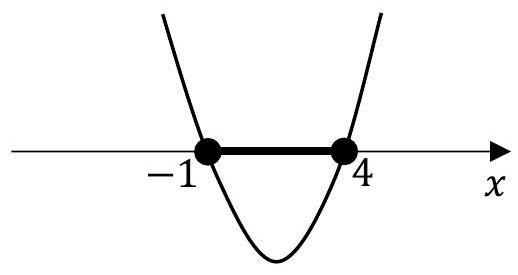
\includegraphics[max width=\textwidth, center]{2025_02_07_7750073b5ff18154e9e8g-17}
\end{itemize}

1 pkt - obliczenie lub podanie pierwiastków trójmianu kwadratowego $x^{2}-3 x-4$ :

$$
x_{1}=-1 \text { oraz } x_{2}=4
$$

ALBO

\begin{itemize}
  \item odczytanie z wykresu funkcji $f(x)=x^{2}-3 x-4$ i zapisanie miejsc zerowych $x_{1}=-1$ oraz $x_{2}=4$.
\end{itemize}

0 pkt - rozwiązanie, w którym zastosowano niepoprawną metodę, albo brak rozwiązania.

\section*{Uwagi:}
\begin{enumerate}
  \item Jeżeli zdający, realizując pierwszy etap rozwiązania zadania, popełni błędy (ale otrzyma dwa różne pierwiastki) i konsekwentnie do popełnionych błędów zapisze zbiór rozwiązań nierówności, to otrzymuje 1 punkt za całe rozwiązanie.
  \item Jeżeli zdający wyznacza pierwiastki trójmianu kwadratowego w przypadku, gdy błędnie obliczony przez zdającego wyróżnik $\Delta$ jest ujemny, to otrzymuje $\mathbf{0}$ punktów za całe rozwiązanie.
  \item Jeżeli zdający, rozpoczynając realizację pierwszego etapu rozwiązania, rozpatruje inny niż podany w zadaniu trójmian kwadratowy, który nie wynika z błędu przekształcenia (np. $x^{2}-4$ ), i w konsekwencji rozpatruje inną nierówność (np. $x^{2}-4 \leq 0$ ), to oznacza, że nie podjął realizacji 1. etapu rozwiązania i otrzymuje $\mathbf{0}$ punktów za całe rozwiązanie.
  \item Akceptowane jest zapisanie pierwiastków trójmianu w postaci $a+b \sqrt{c}$, gdzie $a, b, c$ są liczbami wymiernymi.
  \item Jeżeli zdający poda zbiór rozwiązań w postaci graficznej z poprawnie zaznaczonymi końcami przedziałów oraz zapisze: $x \in(-1,4)$, to otrzymuje 1 punkt za całe rozwiązanie.
\end{enumerate}

\section*{Kryteria uwzględniające specyficzne trudności w uczeniu się matematyki}
Jeśli zdający pomyli porządek liczb na osi liczbowej, np. zapisze zbiór rozwiązań nierówności $w$ postaci $\langle 4,-1\rangle$, to otrzymuje 2 punkty.

\section*{Przykładowe pełne rozwiązanie}
Zapisujemy nierówność w postaci $x^{2}-3 x-4 \leq 0$ i obliczamy pierwiastki trójmianu $x^{2}-3 x-4$.\\
Obliczamy wyróżnik trójmianu: $\Delta=25$\\
i obliczamy jego pierwiastki: $x_{1}=-1$ oraz $x_{2}=4$\\
ALBO\\
podajemy pierwiastki trójmianu bezpośrednio, zapisując je lub zaznaczając je na wykresie:\\
$x_{1}=-1$ oraz $x_{2}=4$.\\
Podajemy zbiór rozwiązań nierówności: $\langle-1,4\rangle$ lub $x \in\langle-1,4\rangle$, lub zaznaczamy zbiór rozwiązań na osi liczbowej:\\
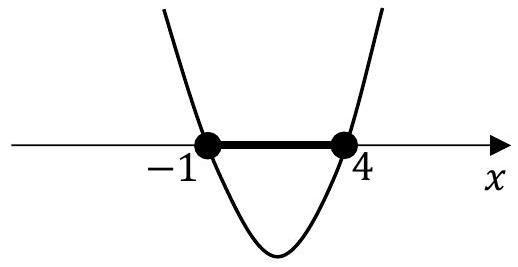
\includegraphics[max width=\textwidth, center]{2025_02_07_7750073b5ff18154e9e8g-18}

Zadanie 31. (0-2)

\begin{center}
\begin{tabular}{|l|l|}
\hline
\multicolumn{2}{|c|}{Wymagania egzaminacyjne 2024} \\
\hline
\multicolumn{1}{|c|}{Wymaganie ogólne} & \multicolumn{1}{|c|}{Wymaganie szczegółowe} \\
\hline
V. Rozumowanie i argumentacja. & Zdający: \\
 & \begin{tabular}{l}
2. używa wzorów skróconego mnożenia na \\
 \\
 \\
 \\
\end{tabular}$\left(\begin{array}{l}\text { n })^{2} \text { oraz } a^{2}-b^{2} .\end{array}\right.$ \\
\hline
\end{tabular}
\end{center}

\section*{Zasady oceniania}
2 pkt - przekształcenie nierówności $(3 x+y)(x+3 y)>16 x y$ do postaci\\
$c(x-y)^{2}>0$, gdzie $c>0\left(\right.$ np. $\left.3(x-y)^{2}>0\right)$\\
lub\\
$c(x-y)^{2}<0$, gdzie $c<0$ (np. $-3(x-y)^{2}<0$ ),\\
lub\\
$(c x-c y)^{2}>0$, gdzie $c \neq 0$ (np. $\left.(\sqrt{3} x-\sqrt{3} y)^{2}>0\right)$\\
oraz powołanie się na założenie i stwierdzenie, że kwadrat każdej liczby rzeczywistej różnej od zera jest liczbą dodatnią\\
ALBO

\begin{itemize}
  \item przekształcenie nierówności $(3 x+y)(x+3 y)>16 x y$ do postaci $x^{2}+y^{2}>2 x y$ oraz powołanie się na nierówność $x^{2}+y^{2} \geq 2 x y$ i stwierdzenie, że dla $x \neq y$ nierówność jest ostra,\\
ALBO
  \item obliczenie wyróżnika trójmianu kwadratowego $3 x^{2}-6 x y+3 y^{2}$ zmiennej $x$ oraz uzasadnienie, że funkcja $f(x)=3 x^{2}-6 x y+3 y^{2}$ przyjmuje wartości dodatnie dla $x \neq y$,\\
ALBO
  \item obliczenie wyróżnika trójmianu kwadratowego $3 y^{2}-6 x y+3 x^{2}$ zmiennej $y$ oraz uzasadnienie, że funkcja $f(y)=3 y^{2}-6 x y+3 x^{2}$ przyjmuje wartości dodatnie dla $y \neq x$.
\end{itemize}

1 pkt - przekształcenie nierówności $(3 x+y)(x+3 y)>16 x y$ do postaci\\
$3 x^{2}-6 x y+3 y^{2}>0$\\
ALBO

\begin{itemize}
  \item przekształcenie nierówności $(3 x+y)(x+3 y)>16 x y$ do postaci $x^{2}+y^{2}>2 x y$, ALBO
  \item obliczenie wyróżnika trójmianu kwadratowego $3 x^{2}-6 x y+3 y^{2}$ zmiennej $x$, ALBO,
  \item obliczenie wyróżnika trójmianu kwadratowego $3 y^{2}-6 x y+3 x^{2}$ zmiennej $y$.
\end{itemize}

0 pkt - rozwiązanie, w którym zastosowano niepoprawną metodę, albo brak rozwiązania.

\section*{Uwaga:}
Jeśli zdający sprawdza prawdziwość nierówności tylko dla wybranych wartości $x$ i $y$, to otrzymuje $\mathbf{0}$ punktów za całe rozwiązanie.

\section*{Przykładowe pełne rozwiązania}
Sposób 1\\
Przekształcamy nierówność $(3 x+y)(x+3 y)>16 x y$ w sposób równoważny:

$$
3 x^{2}-6 x y+3 y^{2}>0
$$

Zauważamy, że lewą stronę nierówności można zapisać w postaci

$$
3(x-y)^{2}>0
$$

Z założenia wiadomo, że $x \neq y$, więc $3(x-y)^{2}$ jest liczbą dodatnią.\\
To należało wykazać.

\section*{Sposób II (trójmian kwadratowy zmiennej $x$ z parametrem y)}
Przekształcamy równoważnie nierówność $(3 x+y)(x+3 y)>16 x y$ i otrzymujemy

$$
3 x^{2}-6 x y+3 y^{2}>0
$$

Wyrażenie $3 x^{2}-6 x y+3 y^{2}$ traktujemy jako trójmian kwadratowy zmiennej $x$. Obliczamy wyróżnik $\Delta$ trójmianu:

$$
\Delta=(-6 y)^{2}-4 \cdot 3 \cdot 3 y^{2}=0
$$

Funkcja $f(x)=3 x^{2}-6 x y+3 y^{2}$ ma dokładnie jedno miejsce zerowe: $x=y$. Ponieważ współczynnik przy drugiej potędze zmiennej jest dodatni, więc żaden fragment wykresu funkcji $f$ nie leży poniżej osi odciętych. Zatem funkcja $f$ przyjmuje wartości dodatnie dla każdego $x \neq y$.

Oznacza to, że dla każdej liczby rzeczywistej $x$ i dla każdej liczby rzeczywistej $y \neq x$ nierówność $3 x^{2}-6 x y+3 y^{2}>0$ jest prawdziwa.\\
Zatem nierówność $(3 x+y)(x+3 y)>16 x y$ również jest prawdziwa dla każdej liczby rzeczywistej $x$ i dla każdej liczby rzeczywistej $y \neq x$. To należało wykazać.

Zadanie 32. (0-2)

\begin{center}
\begin{tabular}{|l|l|}
\hline
\multicolumn{2}{|c|}{Wymagania egzaminacyjne 2024} \\
\hline
\multicolumn{1}{|c|}{Wymaganie ogólne} & \multicolumn{1}{c|}{Wymaganie szczegółowe} \\
\hline
IV. Użycie i tworzenie strategii. & \begin{tabular}{l}
Zdajacy: \\
4.9) wyznacza wzór funkcji kwadratowej na \\
podstawie pewnych informacji o tej funkcji \\
lub o jej wykresie. \\
\end{tabular} \\
\hline
\end{tabular}
\end{center}

\section*{Zasady oceniania}
2 pkt - zastosowanie poprawnej metody i obliczenie współczynników: $b=4, c=-5$.\\
1 pkt - zapisanie drugiego miejsca zerowego funkcji $f: x_{2}=-5$\\
ALBO

\begin{itemize}
  \item obliczenie drugiej współrzędnej wierzchołka paraboli będącej wykresem funkcji $f$ :\\
$q=-9$,\\
ALBO
  \item obliczenie współczynnika $b: b=4$.
\end{itemize}

0 pkt - rozwiązanie, w którym zastosowano niepoprawną metodę, albo brak rozwiązania.

\section*{Przykładowe pełne rozwiązania}
\section*{Sposób 1}
Wykres funkcji $f$ jest symetryczny względem prostej o równaniu $x=-2$, zatem drugie miejsce zerowe jest równe $x_{2}=-5$.\\
Wzór funkcji $f$ zapisujemy w postaci iloczynowej $f(x)=(x-1)(x+5)$, a następnie w postaci ogólnej $f(x)=x^{2}+4 x-5$.\\
Zatem współczynniki $b$ i $c$ są równe: $b=4, c=-5$.

\section*{Sposób II}
Wykres funkcji $f$ jest symetryczny względem prostej o równaniu $x=-2$, zatem pierwsza współrzędna wierzchołka paraboli będącej wykresem funkcji $f$ jest równa $p=-2$.\\
Wzór funkcji $f$ zapisujemy w postaci kanonicznej $f(x)=(x+2)^{2}+q$.\\
Punkt $(1,0)$ leży na wykresie funkcji $f$, zatem dla argumentu 1 funkcja $f$ przyjmuje wartość 0 . Stąd otrzymujemy równanie:

$$
0=(1+2)^{2}+q
$$

Zatem $q=-9$.\\
Wzór funkcji $f(x)=(x+2)^{2}-9$ przekształcamy do postaci ogólnej $f(x)=x^{2}+4 x-5$. Zatem współczynniki $b$ i $c$ są równe: $b=4, c=-5$.

\section*{Sposób III}
Wykres funkcji $f$ jest symetryczny względem prostej o równaniu $x=-2$, zatem pierwsza współrzędna wierzchołka paraboli będącej wykresem funkcji $f$ jest równa $p=-2$.\\
Obliczamy współczynnik $b$, korzystając ze wzoru $p=-\frac{b}{2 a}$ :

$$
-2=-\frac{b}{2}
$$

Stąd $b=4$.\\
Punkt $(1,0)$ leży na wykresie funkcji $f$, zatem dla argumentu 1 funkcja $f$ przyjmuje wartość 0 . Stąd otrzymujemy równanie

$$
0=1^{2}+4 \cdot 1+c
$$

Zatem współczynniki $b$ i $c$ są równe: $b=4, c=-5$.

Zadanie 33. (0-2)

\begin{center}
\begin{tabular}{|c|c|}
\hline
\multicolumn{2}{|c|}{Wymagania egzaminacyjne 2024} \\
\hline
Wymaganie ogólne & Wymaganie szczegółowe \\
\hline
IV. Użycie i tworzenie strategii. & \begin{tabular}{l}
Zdający: \\
5.3) stosuje wzór na $n$-ty wyraz i na sumę $n$ początkowych wyrazów ciągu arytmetycznego. \\
\end{tabular} \\
\hline
\end{tabular}
\end{center}

\section*{Zasady oceniania}
2 pkt - zastosowanie poprawnej metody i obliczenie różnicy ciągu: $r=-2$.\\
1 pkt - zapisanie układu równań pozwalającego obliczyć $r$, np.:

$$
\begin{aligned}
& -1=a_{1}+2 r \text { oraz }-165=\frac{2 a_{1}+14 r}{2} \cdot 15, \\
& -1=a_{1}+2 r \text { oraz } a_{15}=a_{1}+14 r \text { oraz }-165=\frac{a_{1}+a_{15}}{2} \cdot 15, \\
& a_{3}=-1 \text { oraz }-165=\frac{\left(a_{3}-2 r\right)+\left(a_{3}+12 r\right)}{2} \cdot 15
\end{aligned}
$$

ALBO

\begin{itemize}
  \item zapisanie równania $z$ jedną niewiadomą $r$, np.:
\end{itemize}

$$
\begin{aligned}
& (-1-2 r)+(-1-r)+(-1)+(-1+r)+\ldots+(-1+12 r)=-165 \\
& \frac{2(-1-2 r)+14 r}{2} \cdot 15=-165 \\
& \frac{(-1-2 r)+(-1+12 r)}{2} \cdot 15=-165
\end{aligned}
$$

ALBO

\begin{itemize}
  \item obliczenie ósmego wyrazu ciągu ( $a_{n}$ ) z wykorzystaniem własności ciągu arytmetycznego: $a_{8}=-11$ (dla sposobów IV oraz V),
\end{itemize}

\section*{ALBO}
\begin{itemize}
  \item zapisanie kolejnych piętnastu początkowych wyrazów ciągu $\left(a_{n}\right)$ :
\end{itemize}

$$
3,1,-1,-3,-5,-7,-9,-11,-13,-15,-17,-19,-21,-23,-25 \text {. }
$$

0 pkt - rozwiązanie, w którym zastosowano niepoprawną metodę, albo brak rozwiązania.

\section*{Uwagi:}
\begin{enumerate}
  \item Jeżeli zdający myli ciąg arytmetyczny z geometrycznym, to otrzymuje $\mathbf{0}$ punktów za całe rozwiązanie, o ile nie nabył prawa do innej liczby punktów.
  \item Jeżeli zdający zapisze tylko $r=-2$, to otrzymuje 1 punkt za całe rozwiązanie.
  \item Jeżeli zdający błędnie interpretuje liczbę (-165) jako piętnasty wyraz ciągu, to otrzymuje $\mathbf{0}$ punktów za całe rozwiązanie.
\end{enumerate}

\section*{Przykładowe pełne rozwiązania}
\section*{Sposób 1}
Korzystamy ze wzorów na $n$-ty wyraz i sumę $n$ początkowych wyrazów ciągu arytmetycznego i otrzymujemy układ równań

$$
\left\{\begin{array}{c}
-1=a_{1}+2 r \\
-165=\frac{2 a_{1}+14 r}{2} \cdot 15
\end{array}\right.
$$

Przekształcając ten układ równoważnie, otrzymujemy

$$
\left\{\begin{array}{c}
-1=a_{1}+2 r \\
-11=a_{1}+7 r
\end{array}\right.
$$

Odejmując stronami równania układu, otrzymujemy

$$
\begin{aligned}
10 & =-5 r \\
r & =-2
\end{aligned}
$$

Różnica ciągu jest równa ( -2 ).

\section*{Sposób II}
Suma kolejnych piętnastu początkowych wyrazów ciągu arytmetycznego jest równa (-165), zatem

$$
\begin{gathered}
a_{1}+a_{2}+a_{3}+\ldots+a_{15}=-165 \\
\left(a_{3}-2 r\right)+\left(a_{3}-r\right)+a_{3}+\left(a_{3}+r\right)+\left(a_{3}+2 r\right)+\ldots+\left(a_{3}+12 r\right)=-165 \\
15 a_{3}+(-2 r-r+0+r+2 r+3 r+\ldots+12 r)=-165
\end{gathered}
$$

gdzie $a_{3}=-1$, a suma piętnastu liczb $(-2 r-r+0+r+2 r+3 r+\ldots+12 r)$ jest równa

$$
\frac{-2 r+12 r}{2} \cdot 15=75 r
$$

Zatem

$$
\begin{gathered}
15 \cdot(-1)+75 r=-165 \\
75 r=-150 \\
r=-2
\end{gathered}
$$

Różnica ciągu jest równa (-2).

\section*{Sposób III}
Suma kolejnych piętnastu początkowych wyrazów ciągu arytmetycznego jest równa ( -165 ), zatem

$$
\begin{gathered}
\frac{a_{1}+a_{15}}{2} \cdot 15=-165 \\
a_{1}+a_{15}=-22 \\
\left(a_{3}-2 r\right)+\left(a_{3}+12 r\right)=-22 \\
2 a_{3}+10 r=-22
\end{gathered}
$$

Stąd iz tego, że $a_{3}=-1$, otrzymujemy

$$
2 \cdot(-1)+10 r=-22
$$

Zatem

$$
\begin{aligned}
10 r & =-20 \\
r & =-2
\end{aligned}
$$

Różnica ciągu jest równa ( -2 ).

Sposób IV\\
Suma kolejnych piętnastu początkowych wyrazów ciągu arytmetycznego jest równa (-165), zatem

$$
\begin{gathered}
a_{1}+a_{2}+a_{3}+\ldots+a_{15}=-165 \\
\left(a_{8}-7 r\right)+\left(a_{8}-6 r\right)+\ldots+a_{8}+\ldots+\left(a_{8}+6 r\right)+\left(a_{8}+7 r\right)=-165 \\
15 a_{8}=-165 \\
a_{8}=\frac{-165}{15}=-11
\end{gathered}
$$

Korzystamy z własności ciągu arytmetycznego i otrzymujemy

$$
\begin{gathered}
a_{8}=a_{3}+5 r \\
-11=-1+5 r \\
r=-2
\end{gathered}
$$

Różnica ciągu jest równa ( -2 ).

\section*{Sposób V}
Korzystamy z własności ciągu arytmetycznego i otrzymujemy równania:

$$
\begin{aligned}
& a_{8}=\frac{a_{7}+a_{9}}{2} \\
& a_{8}=\frac{a_{6}+a_{10}}{2} \\
& a_{8}=\frac{a_{5}+a_{11}}{2} \\
& a_{8}=\frac{a_{4}+a_{12}}{2} \\
& a_{8}=\frac{a_{3}+a_{13}}{2} \\
& a_{8}=\frac{a_{2}+a_{14}}{2} \\
& a_{8}=\frac{a_{1}+a_{15}}{2}
\end{aligned}
$$

Zatem

$$
\begin{aligned}
a_{1}+a_{2}+\ldots+a_{14}+a_{15} & =\left(a_{1}+a_{15}\right)+\left(a_{2}+a_{14}\right)+\ldots+\left(a_{7}+a_{9}\right)+a_{8}= \\
& =15 a_{8}=-165
\end{aligned}
$$

Stąd $a_{8}=-11$. Ponieważ

$$
a_{8}=a_{3}+5 r
$$

więc otrzymujemy

$$
\begin{gathered}
-11=-1+5 r \\
r=-2
\end{gathered}
$$

Różnica ciągu jest równa (-2).

Zadanie 34. (0-2)

\begin{center}
\begin{tabular}{|l|l|}
\hline
\multicolumn{2}{|c|}{Wymagania egzaminacyjne 2024} \\
\hline
\multicolumn{1}{|c|}{Wymaganie ogólne} & \multicolumn{1}{c|}{Wymagania szczegółowe} \\
\hline
IV. Użycie i tworzenie strategii. & Zdający: \\
 & 8.5) wyznacza współrzędne środka odcinka; \\
 & 8.6) oblicza odległość dwóch punktów. \\
\hline
\end{tabular}
\end{center}

\section*{Zasady oceniania}
2 pkt - zastosowanie poprawnej metody i obliczenie długości boku $B C$ : $|B C|=\sqrt{52}$.\\
1 pkt - zapisanie współrzędnych punktu $C: C=(14,8)$\\
ALBO

\begin{itemize}
  \item zapisanie współrzędnych punktu $D: D=(2,12)$, ALBO
  \item zapisanie współrzędnych środka $S$ boku $A B: S=(4,4)$ oraz zapisanie równości $|B C|=2|P S|$,\\
ALBO
  \item zapisanie równości $\overrightarrow{C B}=2 \cdot \overrightarrow{P A}+\overrightarrow{A B}$ oraz obliczenie wspórrzędnych wektorów $\overrightarrow{P A}$; $\overrightarrow{A B}: \overrightarrow{P A}=[-8,-1]$ oraz $\overrightarrow{A B}=[12,-4]$, ALBO
  \item obliczenie długości odcinków $A B, A P$ oraz $B P$ i cosinusa kąta $\alpha$ oraz cosinusa kąta $\left(180^{\circ}-\alpha\right)$, gdzie $\alpha=|\Varangle A P B|:|A B|=4 \sqrt{10}$ oraz $|A P|=\sqrt{65}$, oraz $|B P|=\sqrt{41}$, oraz $\cos \alpha=-\frac{27}{\sqrt{65} \cdot \sqrt{41}}$, oraz $\cos \left(180^{\circ}-\alpha\right)=\frac{27}{\sqrt{65} \cdot \sqrt{41}}$.
\end{itemize}

0 pkt - rozwiązanie, w którym zastosowano niepoprawną metodę, albo brak rozwiązania.

\section*{Uwagi:}
\begin{enumerate}
  \item Jeżeli zdający korzysta z punktów kratowych oraz błędnie zaznaczy w układzie współrzędnych co najmniej jeden z punktów $A, B, C, P$ i na tej podstawie oblicza długość odcinka $B C$, to otrzymuje $\mathbf{0}$ punktów za całe rozwiązanie (o ile nie nabył praw do innej punktacji).
  \item Jeżeli zdający korzysta z punktów kratowych oraz poprawnie zaznaczy w układzie współrzędnych punkty $A, B, C, P$, lecz błędnie odczyta współrzędne jednego z tych punktów, i na tej podstawie oblicza długość odcinka $B C$, to otrzymuje 1 punkt za całe rozwiązanie.
  \item Jeżeli zdający obliczy długość odcinka $B C$, korzystając z przybliżonych wartości funkcji trygonometrycznych, to może otrzymać co najwyżej 1 punkt za całe rozwiązanie.
\end{enumerate}

\section*{Przykładowe pełne rozwiązania}
Sposób 1\\
Punkt $P$ jest środkiem przekątnej $A C$. Ze wzoru na współrzędne środka odcinka otrzymujemy

$$
\frac{-2+x_{c}}{2}=6 \quad \text { oraz } \quad \frac{6+y_{c}}{2}=7
$$

Zatem $C=(14,8)$.\\
Obliczamy długość odcinka $B C$ :

$$
|B C|=\sqrt{(14-10)^{2}+(8-2)^{2}}=\sqrt{16+36}=\sqrt{52}=2 \sqrt{13}
$$

\section*{Sposób II}
Punkt $P$ jest środkiem przekątnej $B D$. Ze wzoru na współrzędne środka odcinka otrzymujemy

$$
\frac{10+x_{d}}{2}=6 \quad \text { oraz } \quad \frac{2+y_{d}}{2}=7
$$

Zatem $D=(2,12)$.\\
Obliczamy długość odcinka $B C$ :

$$
|B C|=|A D|=\sqrt{(2+2)^{2}+(12-6)^{2}}=\sqrt{16+36}=\sqrt{52}=2 \sqrt{13}
$$

\section*{Sposób III}
Obliczamy współrzędne punktu $S$ środka odcinka $A B$ :

$$
\begin{gathered}
S=\left(\frac{-2+10}{2}, \frac{6+2}{2}\right) \\
S=(4,4)
\end{gathered}
$$

Obliczamy długość odcinka $B C$ :

$$
|B C|=2|P S|=2 \sqrt{(4-6)^{2}+(4-7)^{2}}=2 \sqrt{4+9}=2 \sqrt{13}
$$

Zadanie 35. (0-2)

\begin{center}
\begin{tabular}{|l|l|}
\hline
\multicolumn{2}{|c|}{Wymagania egzaminacyjne 2024} \\
\hline
\multicolumn{1}{|c|}{Wymaganie ogólne} & \multicolumn{1}{c|}{Wymaganie szczegółowe} \\
\hline
III. Modelowanie matematyczne. & Zdający: \\
 & 10.2) oblicza prawdopodobieństwa \\
 & w prostych sytuacjach, stosując klasyczną \\
 & definicję prawdopodobieństwa. \\
\hline
\end{tabular}
\end{center}

\section*{Zasady oceniania}
2 pkt - zastosowanie poprawnej metody obliczenia prawdopodobieństwa zdarzenia $A$ i uzyskanie poprawnego wyniku: $P(A)=\frac{13}{25}$.

1 pkt - wypisanie wszystkich zdarzeń elementarnych lub obliczenie/podanie liczby tych zdarzeń: $|\Omega|=5 \cdot 5$ lub sporządzenie tabeli o 25 polach odpowiadających zdarzeniom elementarnym, z których co najmniej jedno pole jest wypełnione, lub sporządzenie pełnego drzewa stochastycznego ALBO

\begin{itemize}
  \item wypisanie (lub zaznaczenie w tabeli) wszystkich zdarzeń elementarnych sprzyjających zdarzeniu $A$ i niewypisanie żadnego niewłaściwego, ALBO
  \item podanie liczby wszystkich zdarzeń elementarnych sprzyjających zdarzeniu $A$ : $|A|=13$, o ile nie zostały zliczone błędne pary, ALBO
  \item sporządzenie fragmentu drzewa stochastycznego, które zawiera wszystkie gałęzie sprzyjające zdarzeniu $A$ oraz zapisanie prawdopodobieństwa na co najmniej jednym odcinku każdego z etapów doświadczenia, ALBO
  \item podanie prawdopodobieństwa jednoelementowego zdarzenia (elementarnego): $\frac{1}{25}$, ALBO
  \item zapisanie tylko $P(A)=\frac{13}{25}$.
\end{itemize}

0 pkt - rozwiązanie, w którym zastosowano niepoprawną metodę, albo brak rozwiązania.

\section*{Uwagi:}
\begin{enumerate}
  \item Jeżeli zdający zapisuje tylko liczby 13 lub 25 i $z$ rozwiązania nie wynika znaczenie tych liczb, to otrzymuje 0 punktów za całe rozwiązanie.
  \item Jeżeli zdający rozważa losowanie bez zwracania, to otrzymuje $\mathbf{0}$ punktów.
\end{enumerate}

\section*{Przykładowe pełne rozwiązania}
\section*{Sposób 1}
Zdarzeniami elementarnymi są wszystkie uporządkowane pary liczb $(x, y)$, gdzie $x, y \in\{5,6,7,8,9\}$.\\
Liczbę wszystkich zdarzeń elementarnych obliczamy, korzystając z reguły mnożenia.\\
Moc zbioru $\Omega$ jest równa $5 \cdot 5=25$.\\
Liczbę wszystkich zdarzeń elementarnych sprzyjających zdarzeniu $A$ obliczamy, korzystając z reguły mnożenia i reguły dodawania. Suma dwóch liczb naturalnych jest liczbą parzystą, gdy sumujemy dwie liczby parzyste lub dwie liczby nieparzyste. Stąd moc zbioru $A$ jest równa $3 \cdot 3+2 \cdot 2=13$.\\
Zatem prawdopodobieństwo zdarzenia $A$ jest równe $\frac{13}{25}$.

\section*{Sposób II}
W tabeli literą $A$ zaznaczamy zdarzenia elementarne sprzyjające zdarzeniu $A$ (pary liczb, których suma jest liczbą parzystą).

\begin{center}
\begin{tabular}{|c|c|c|c|c|c|}
\hline
 & 5 & 6 & 7 & 8 & 9 \\
\hline
5 & $A$ &  & $A$ &  & $A$ \\
\hline
6 &  & $A$ &  & $A$ &  \\
\hline
7 & $A$ &  & $A$ &  & $A$ \\
\hline
8 &  & $A$ &  & $A$ &  \\
\hline
9 & $A$ &  & $A$ &  & $A$ \\
\hline
\end{tabular}
\end{center}

Moc zbioru $\Omega$ jest równa 25.\\
Zdarzeń sprzyjających wylosowaniu liczb, których suma jest parzysta, jest 13.\\
Zatem prawdopodobieństwo zdarzenia $A$ jest równe $\frac{13}{25}$.

\section*{Sposób III (drzewo stochastyczne)}
Rysujemy drzewo stochastyczne rozważanego doświadczenia.\\
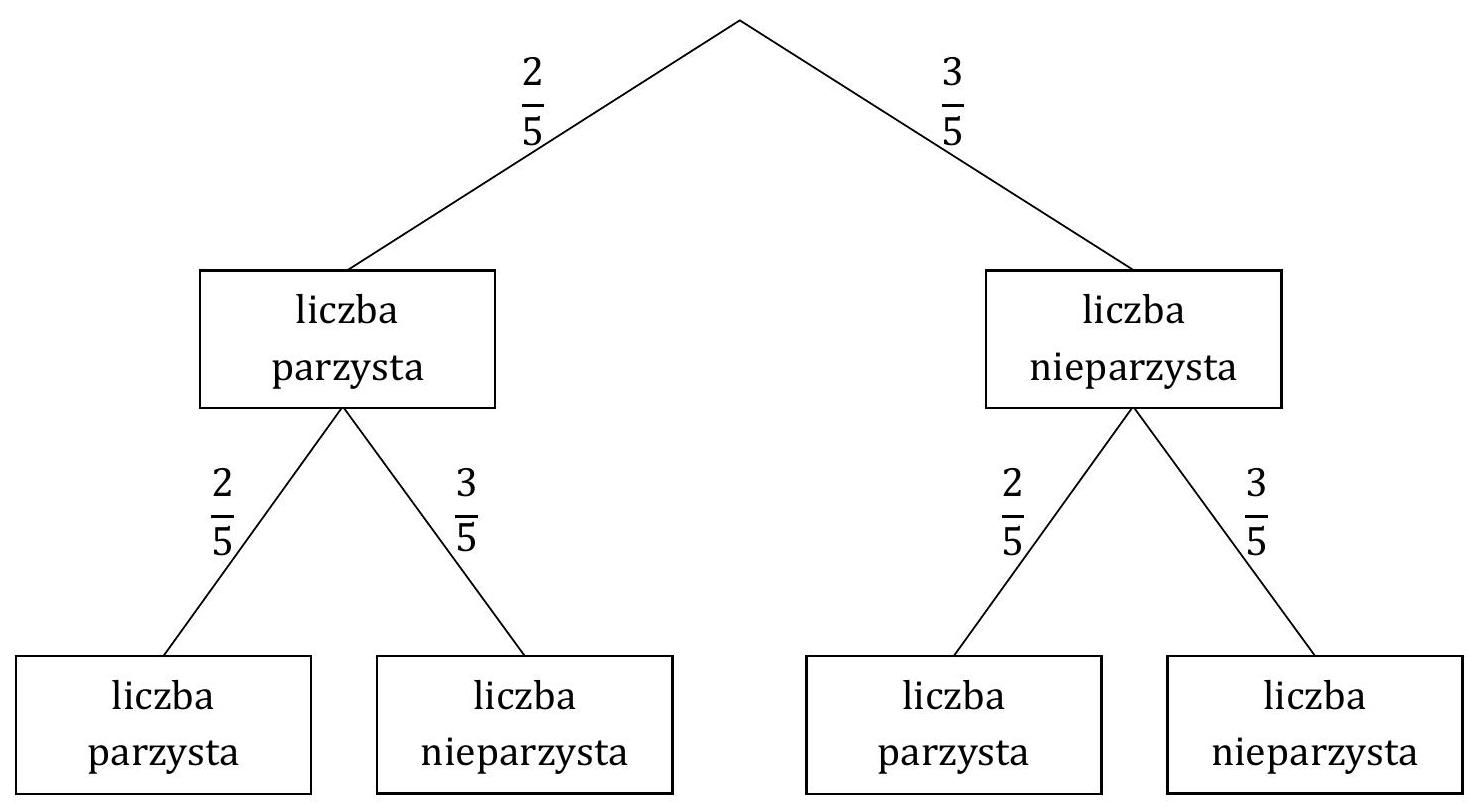
\includegraphics[max width=\textwidth, center]{2025_02_07_7750073b5ff18154e9e8g-31}

Prawdopodobieństwo zdarzenia $A$ jest równe

$$
P(A)=\frac{2}{5} \cdot \frac{2}{5}+\frac{3}{5} \cdot \frac{3}{5}=\frac{13}{25}
$$

Zadanie 36. (0-5)

\begin{center}
\begin{tabular}{|l|l|}
\hline
\multicolumn{2}{|c|}{Wymagania egzaminacyjne 2024} \\
\hline
\multicolumn{1}{|c|}{Wymaganie ogólne} & \multicolumn{1}{c|}{Wymagania szczegółowe} \\
\hline
IV. Użycie i tworzenie strategii. & Zdający: \\
 & G11.2) oblicza pole powierzchni i objętość \\
 & graniastosłupa prostego [...]. \\
 & 9.2) rozpoznaje w graniastosłupach kąt \\
 & między odcinkami i płaszczyznami [...]. \\
\hline
\end{tabular}
\end{center}

\section*{Zasady oceniania}
Część I (Obliczenie cosinusa kąta $\alpha$ )\\
2 pkt - obliczenie cosinusa kąta $\alpha$ : $\cos \alpha=\frac{1}{3}$.\\
1 pkt - zapisanie przekątnej graniastosłupa jako $3 a \sqrt{2}$\\
ALBO

\begin{itemize}
  \item obliczenie tangensa kąta $\alpha$ nachylenia przekątnej graniastosłupa do płaszczyzny podstawy: $\operatorname{tg} \alpha=\frac{4}{\sqrt{2}}$,\\
ALBO
  \item obliczenie długości przekątnej graniastosłupa podobnego do rozpatrywanego.
\end{itemize}

0 pkt - rozwiązanie, w którym zastosowano niepoprawną metodę, albo brak rozwiązania.

\section*{Uwaga:}
Jeżeli zdający obliczy wartość cosinusa kąta $\alpha$, popełniając błąd, który nie jest rachunkowy (np. przyjmie, że przekątna podstawy jest równa $\frac{a \sqrt{3}}{2}$ ), to otrzymuje za tę część rozwiązania 0 punktów, o ile nie nabył praw do innej punktacji.

Część II (Obliczenie pola powierzchni całkowitej graniastosłupa)\\
3 pkt - obliczenie pola powierzchni całkowitej graniastosłupa: $P_{c}=162$.

2 pkt - zapisanie równania z jedną niewiadomą a lub $H$, np.:

$$
a^{2} \cdot 4 a=108,\left(\frac{1}{4} H\right)^{2} \cdot H=108
$$

ALBO

\begin{itemize}
  \item obliczenie skali $k$ podobieństwa graniastosłupa podobnego do rozpatrywanego (gdzie $k \neq 1$ ).
\end{itemize}

1 pkt - zapisanie związku pomiędzy krawędzią podstawy a wysokością graniastosłupa, np.:\\
$H=4 a, a^{2} \cdot H=108$\\
ALBO

\begin{itemize}
  \item obliczenie objętości i pola powierzchni całkowitej graniastosłupa podobnego do rozpatrywanego w skali $k \neq 1$\\
(np. przyjmując $a=1, H=4$ i wtedy $V=4$ oraz $P_{c}=18$ ), ALBO
  \item zapisanie zależności między objętością danego graniastosłupa i graniastosłupa do niego podobnego, np. $108=1^{2} \cdot 4 \cdot k^{3}$ (gdzie $k$ to skala podobieństwa).
\end{itemize}

0 pkt - rozwiązanie, w którym zastosowano niepoprawną metodę, albo brak rozwiązania.

\section*{Przykładowe pełne rozwiązania}
\section*{Sposób 1}
Przyjmujemy oznaczenia:\\
$a$ - długość krawędzi podstawy ( $a>0$ ),\\
$H$ - wysokość graniastosłupa ( $H>0$ ).

Stosunek długości krawędzi podstawy do wysokości graniastosłupa jest równy $\frac{1}{4}$. Zatem $H=4 a$. Objętość graniastosłupa wynosi 108 , stąd otrzymujemy równanie:

$$
\begin{gathered}
a^{2} \cdot 4 a=108 \\
4 a^{3}=108 \\
a^{3}=27 \\
a=3
\end{gathered}
$$

Następnie obliczamy wysokość graniastosłupa, pole powierzchni całkowitej oraz przekątną podstawy:

$$
\begin{gathered}
H=4 \cdot 3=12 \\
P_{c}=2 \cdot a^{2}+4 \cdot a H=2 \cdot 3^{2}+4 \cdot 3 \cdot 12=18+144=162 \\
a \sqrt{2}=3 \sqrt{2}
\end{gathered}
$$

Korzystając z twierdzenia Pitagorasa, obliczamy długość $d$ przekątnej graniastosłupa:

$$
\begin{gathered}
d^{2}=12^{2}+(3 \sqrt{2})^{2}, \text { gdzie } d>0 \\
d^{2}=162 \\
d=\sqrt{162}=9 \sqrt{2}
\end{gathered}
$$

Obliczamy $\cos \alpha$ :

$$
\cos \alpha=\frac{a \sqrt{2}}{d}=\frac{3 \sqrt{2}}{9 \sqrt{2}}=\frac{1}{3}
$$

\section*{Sposób II}
Przyjmujemy oznaczenia:\\
$a$ - długość krawędzi podstawy ( $a>0$ ),\\
$H$ - wysokość graniastosłupa ( $H>0$ ).\\
Stosunek długości krawędzi podstawy do wysokości graniastosłupa jest równy $\frac{1}{4}$. Zatem $H=4 a$. Przekątna podstawy ma długość $a \sqrt{2}$, stąd otrzymujemy:

$$
\operatorname{tg} \alpha=\frac{4 a}{a \sqrt{2}}=2 \sqrt{2}
$$

Zatem $\frac{\sin \alpha}{\cos \alpha}=2 \sqrt{2}$. Stąd $\sin \alpha=2 \sqrt{2} \cdot \cos \alpha$.\\
Wykorzystując tę zależność oraz tożsamość $\sin ^{2} \alpha+\cos ^{2} \alpha=1$, otrzymujemy

$$
\begin{gathered}
(2 \sqrt{2} \cdot \cos \alpha)^{2}+\cos ^{2} \alpha=1 \\
8 \cos ^{2} \alpha+\cos ^{2} \alpha=1 \\
9 \cos ^{2} \alpha=1 \\
\cos ^{2} \alpha=\frac{1}{9}
\end{gathered}
$$

Stąd $\cos \alpha=\frac{1}{3}$, ponieważ $\alpha$ jest kątem ostrym.

Objętość graniastosłupa wynosi 108, stąd otrzymujemy równanie:

$$
\begin{gathered}
a^{2} \cdot 4 a=108 \\
4 a^{3}=108 \\
a^{3}=27 \\
a=3
\end{gathered}
$$

Następnie obliczamy pole powierzchni całkowitej graniastosłupa:

$$
P_{c}=2 \cdot a^{2}+4 \cdot a H=2 \cdot a^{2}+4 \cdot a \cdot 4 a=18 \cdot a^{2}=18 \cdot 3^{2}=162
$$

\section*{Sposób III}
Rozważmy graniastosłup prawidłowy czworokątny $G_{1}$ o wysokości 4 i krawędzi podstawy długości 1. Graniastosłup $G_{1}$ jest podobny do danego graniastosłupa, zatem przekątna graniastosłupa $G_{1}$ jest nachylona do płaszczyzny podstawy pod kątem, którego miara jest równa mierze kąta $\alpha$.

Przekątna podstawy graniastosłupa $G_{1}$ ma długość $\sqrt{2}$.\\
Korzystając z twierdzenia Pitagorasa, obliczamy długość $d_{1}$ przekątnej graniastosłupa $G_{1}$ :

$$
\begin{gathered}
d_{1}^{2}=4^{2}+(\sqrt{2})^{2}, \text { gdzie } d_{1}>0 \\
d_{1}^{2}=18 \\
d_{1}=\sqrt{18}=3 \sqrt{2}
\end{gathered}
$$

Obliczamy $\cos \alpha$ :

$$
\cos \alpha=\frac{\sqrt{2}}{3 \sqrt{2}}=\frac{1}{3}
$$

Objętość $V_{1}$ graniastosłupa $G_{1}$ jest równa

$$
V_{1}=1^{2} \cdot 4=4
$$

Pole $P_{c_{1}}$ powierzchni całkowitej graniastosłupa $G_{1}$ jest równe

$$
P_{c_{1}}=2 \cdot 1^{2}+4 \cdot 1 \cdot 4=18
$$

Stosunek objętości $V_{1}$ graniastosłupa $G_{1}$ do objętości $V$ danego graniastosłupa jest równy sześcianowi skali podobieństwa. Zatem

$$
k^{3}=\frac{V_{1}}{V}=\frac{4}{108}=\frac{1}{27}
$$

Stąd $k=\frac{1}{3}$.\\
Stosunek pola $P_{c_{1}}$ powierzchni całkowitej graniastosłupa $G_{1}$ do pola $P_{c}$ powierzchni całkowitej danego graniastosłupa jest równy kwadratowi skali podobieństwa. Zatem

$$
\begin{gathered}
\frac{P_{c_{1}}}{P_{c}}=k^{2} \\
\frac{18}{P_{c}}=\frac{1}{9} \\
P_{c}=18 \cdot 9=162
\end{gathered}
$$

\section*{Ocena prac osób ze stwierdzoną dyskalkulią}
Obowiązują Zasady oceniania stosowane przy sprawdzaniu prac zdających bez stwierdzonej dyskalkulii z dodatkowym uwzględnieniem:\\
a) ogólnych zasad oceniania zadań otwartych w przypadku arkuszy osób ze stwierdzoną dyskalkulią (punkty 1.-12.);\\
b) dodatkowych szczegółowych zasad oceniania zadań otwartych w przypadku arkuszy osób ze stwierdzoną dyskalkulią - egzamin maturalny z matematyki, poziom podstawowy, termin główny 2024.\\
I. Ogólne zasady oceniania zadań otwartych w przypadku arkuszy osób ze stwierdzoną dyskalkulią

\begin{enumerate}
  \item Nie należy traktować jako błędy merytoryczne pomyłek, wynikających z:
\end{enumerate}

\begin{itemize}
  \item błędnego przepisania
  \item przestawienia cyfr
  \item zapisania innej cyfry, ale o podobnym wyglądzie
  \item przestawienia położenia przecinka
  \item przestawienia położenia znaku liczby.
\end{itemize}

\begin{enumerate}
  \setcounter{enumi}{1}
  \item W przypadku błędów, wynikających ze zmiany znaku liczby, należy w każdym zadaniu oddzielnie przeanalizować, czy zdający opanował inne umiejętności, poza umiejętnościami rachunkowymi, oceniane w zadaniu. W przypadku opanowania badanych umiejętności zdający powinien otrzymać przynajmniej 1 punkt.
  \item We wszystkich zadaniach otwartych, w których wskazano poprawną metodę rozwiązania, części lub całości zadania, zdającemu należy przyznać przynajmniej 1 punkt, zgodnie z kryteriami do poszczególnych zadań.
  \item Jeśli zdający przedstawia nieprecyzyjne zapisy, na przykład pomija nawiasy lub zapisuje nawiasy w niewłaściwych miejscach, ale przeprowadza poprawne rozumowanie lub stosuje właściwą strategię, to może otrzymać przynajmniej 1 punkt za rozwiązanie zadania.
  \item W przypadku zadania wymagającego wyznaczenia pierwiastków trójmianu kwadratowego zdający może otrzymać 1 punkt, jeżeli przedstawi poprawną metodę wyznaczania pierwiastków trójmianu kwadratowego, przy podanych w treści zadania wartościach liczbowych.
  \item W przypadku zadania wymagającego rozwiązania nierówności kwadratowej zdający może otrzymać 1 punkt, jeżeli stosuje poprawny algorytm rozwiązywania nierówności kwadratowej, przy podanych w treści zadania wartościach liczbowych.
  \item W przypadku zadania wymagającego stosowania własności funkcji kwadratowej zdający może otrzymać 1 punkt za wykorzystanie konkretnych własności funkcji kwadratowej, istotnych przy poszukiwaniu rozwiązania.
  \item W przypadku zadania wymagającego zastosowania własności ciągów arytmetycznych lub geometrycznych zdający może otrzymać 1 punkt, jeżeli przedstawi wykorzystanie takiej własności ciągu, która umożliwia znalezienie rozwiązania zadania.
  \item W przypadku zadania wymagającego analizowania figur geometrycznych na płaszczyźnie kartezjańskiej zdający może otrzymać punkty, jeżeli przy poszukiwaniu rozwiązania przedstawi poprawne rozumowanie, wykorzystujące własności figur geometrycznych lub zapisze zależności, pozwalające rozwiązać zadanie.
  \item W przypadku zadania z rachunku prawdopodobieństwa zdający może otrzymać przynajmniej 1 punkt, jeśli przy wyznaczaniu liczby zdarzeń elementarnych sprzyjających rozważanemu zdarzeniu przyjmuje określoną regularność lub podaje prawidłową metodę wyznaczenia tej liczby zdarzeń elementarnych.
  \item W przypadku zadania z geometrii zdający może otrzymać przynajmniej 1 punkt, jeżeli podaje poprawną metodę wyznaczenia długości odcinka potrzebnej do znalezienia rozwiązania.
  \item W przypadku zadania wymagającego przeprowadzenia dowodu (z zakresu algebry lub geometrii), jeśli w przedstawionym rozwiązaniu zdający powoła się na własność, która wyznacza istotny postęp, prowadzący do przeprowadzenia dowodu, to może otrzymać 1 punkt.\\
II. Dodatkowe szczegółowe zasady oceniania zadań otwartych w przypadku arkuszy osób ze stwierdzoną dyskalkulią
\end{enumerate}

\section*{Zadanie 30.}
1 pkt - zastosowanie poprawnej metody obliczenia pierwiastków trójmianu kwadratowego $x^{2}-3 x-4$, tzn. zastosowanie wzorów na pierwiastki trójmianu kwadratowego i obliczenie tych pierwiastków\\
ALBO

\begin{itemize}
  \item konsekwentne (do otrzymanego w wyniku popełnienia błędów o charakterze dyskalkulicznym ujemnego wyróżnika) narysowanie paraboli, ALBO
  \item poprawne rozwiązanie nierówności $x^{2}-4 \leq 0$ (tzn. stosuje się punkt 6. ogólnych zasad oceniania), ALBO
  \item konsekwentne (do wyznaczonych przez siebie pierwiastków oraz rozpatrywanego trójmianu i nierówności) wyznaczenie zbioru rozwiązań nierówności.
\end{itemize}

\section*{Uwagi:}
\begin{enumerate}
  \item Jeżeli zdający, rozwiązując nierówność, pomyli porządek liczb na osi liczbowej i zapisze zbiór rozwiązań nierówności w postaci $\langle 4,-1\rangle$, to może otrzymać $\mathbf{2}$ punkty za całe rozwiązanie.
  \item Nie stosuje się uwag 2. i 3. z zasad oceniania arkusza standardowego.
\end{enumerate}

\section*{Zadanie 31.}
1 pkt - przekształcenie wyrażenia $(3 x+y)(x+3 y)$ do postaci $3 x^{2}+9 x y+x y+3 y^{2}$.

\section*{Zadanie 32.}
Stosuje się zasady oceniania arkusza standardowego.

\section*{Zadanie 33.}
1 pkt - zapisanie równania z dwiema niewiadomymi, gdzie jedną z niewiadomych jest różnica ciągu arytmetycznego, np .: $-1=a_{1}+2 r,-165=\frac{2 a_{1}+14 r}{2} \cdot 15$.

\section*{Zadanie 34.}
1 pkt - poprawne zaznaczenie w kartezjańskim układzie współrzędnych punktu $C$ ALBO

\begin{itemize}
  \item poprawne zaznaczenie w kartezjańskim układzie współrzędnych punktu $D$, ALBO
  \item zapisanie współrzędnych środka $S$ boku $A B: S=(4,4)$.
\end{itemize}

\section*{Zadanie 35.}
1 pkt - zapisanie jedynie liczby 25 (należy traktować to jako wyznaczenie liczby wszystkich zdarzeń elementarnych).

\section*{Uwagi:}
\begin{enumerate}
  \item W ocenie rozwiązania tego zadania (dla zdających z dyskalkulią) nie stosuje się uwagi 1. ze standardowych zasad oceniania.
  \item Jeżeli zdający poprawnie wypisze/zaznaczy wszystkie zdarzenia elementarne sprzyjające zdarzeniu $A$, lecz popełni błąd w ich zliczeniu (np. $|A|=12$ ) i konsekwentnie zapisze wynik (np. $\frac{12}{25}$ ), to otrzymuje 2 punkty.
\end{enumerate}

\section*{Zadanie 36.}
1 pkt - zapisanie długości krawędzi podstawy oraz wysokości graniastosłupa podobnego do rozpatrywanego (np. $a=1, H=4$ ).


\end{document}